\begin{frame}[label=adapting_gps]
    \frametitle{Adapting GNSS Position Solution for Meteor Radar}
    \begin{columns}
        \begin{column}{0.5\textwidth}
            Meteor radar gives \alert{bistatic range measurements} %
            \begin{itemize} \footnotesize %
                \item Distance from \textcolor{blue}{\textbf{TX}}, to meteor trail, to \textcolor{red}{\textbf{RX}}
            \end{itemize}

            % Each measurement constrains the meteor to an \alert{ellipsoid}
            % \begin{itemize} \footnotesize
            %     \item Foci: \textcolor{blue}{\textbf{TX}}, \textcolor{red}{\textbf{RX}}
            %     \item Major axis = bistatic range
            % \end{itemize}

            Using \textcolor{cyan}{\textbf{RX}\textsubscript{1}}, \textcolor{magenta}{\textbf{RX}\textsubscript{2}}, \textcolor{yellow}{\textbf{RX}\textsubscript{3}}, {\textbf{RX}\textsubscript{4}}:
            {\setlength{\leftmargini}{1em} \begin{itemize} \footnotesize
                \item<2->[\(\blacktriangleright\)] 1 bistatic range measurement constrains position to an \alert{ellipsoid} 
                \item<3->[{\(\blacktriangleright\)}] 2 measurements \(\xrightarrow[]{}\) \alert{ellipse} 
                \item<4->[{\(\blacktriangleright\)}] 3 measurements \(\xrightarrow[]{}\) \alert{2 points}
                \item<5->[\(\blacktriangleright\)] 4 measurements \(\xrightarrow[]{}\) \alert{1 point}!
            \end{itemize}}
        \end{column}
        \begin{column}{0.6\textwidth}
            \begin{tikzpicture}[remember picture,overlay]
                \node<1>[anchor=east] at ([yshift=-0.35cm]current page.east) {
                    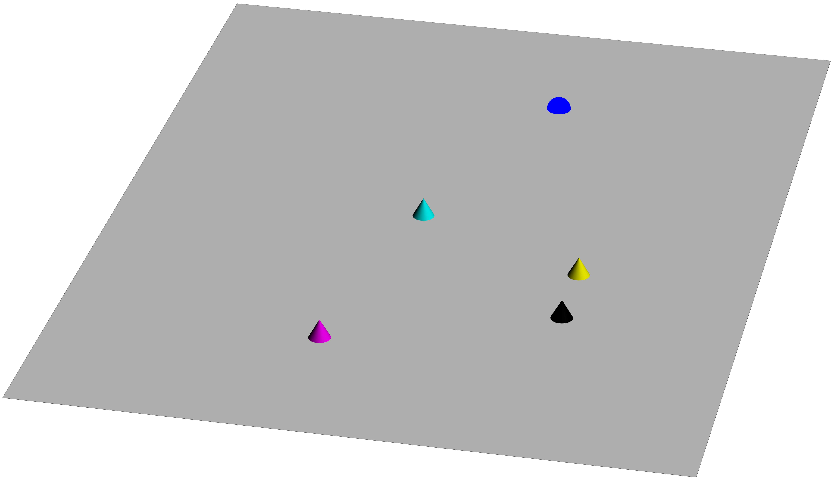
\includegraphics[width=\linewidth]{img/0ellipsoids.pdf}%
                };
                \node<2>[anchor=east] at (current page.east) {
                    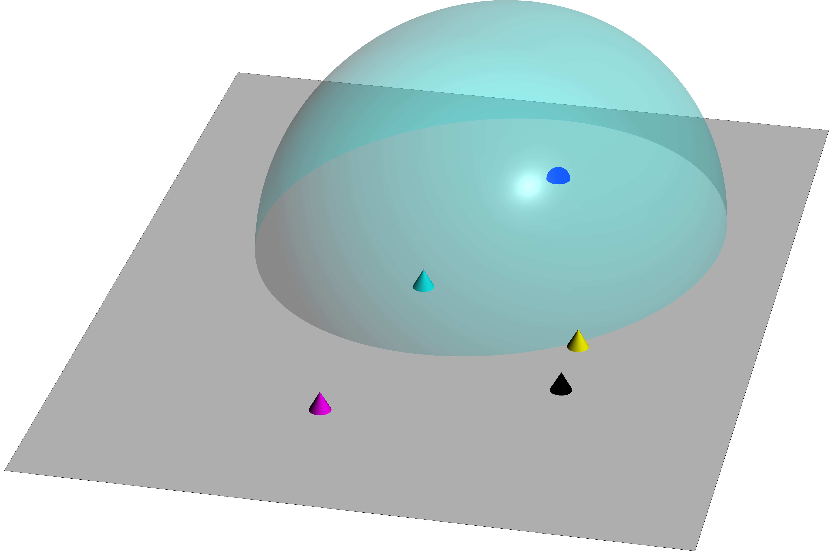
\includegraphics[width=\linewidth]{img/1ellipsoids.pdf}%
                };
                \node<3>[anchor=east] at (current page.east) {
                    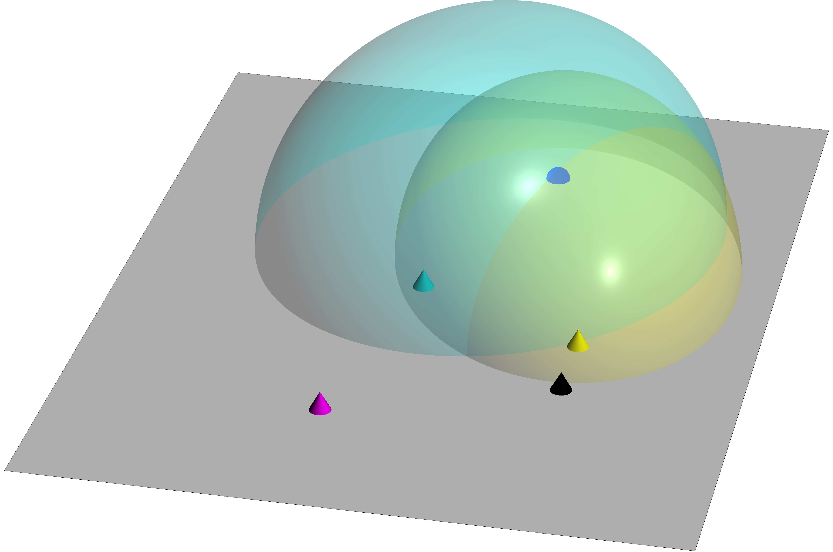
\includegraphics[width=\linewidth]{img/2ellipsoids.pdf}%
                };
                \node<4>[anchor=east] at (current page.east) {
                    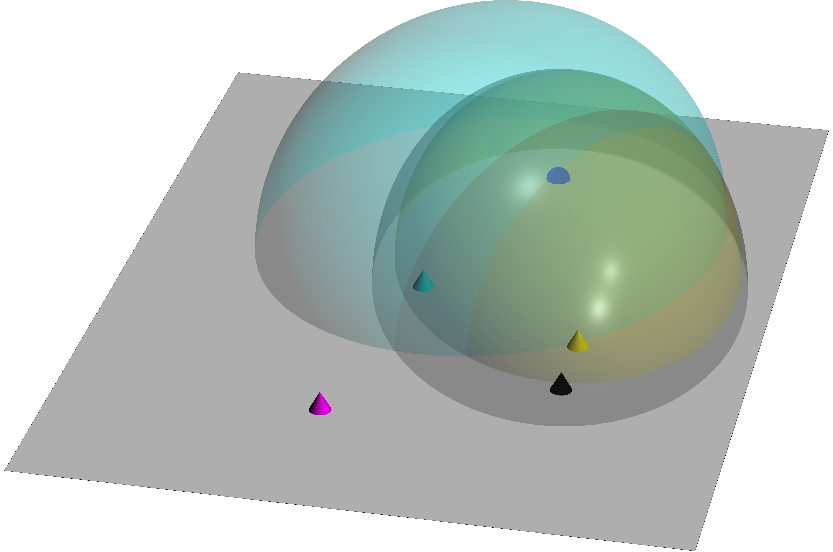
\includegraphics[width=\linewidth]{img/3ellipsoids.pdf}%
                };
                \node<5->[anchor=east] at ([yshift=-0.15cm]current page.east) {
                    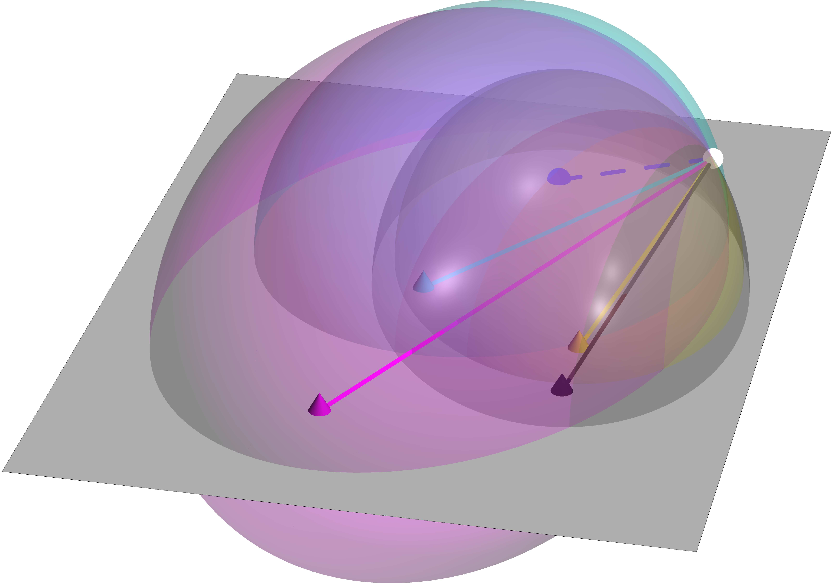
\includegraphics[width=\linewidth]{img/4ellipsoids.pdf}%
                };
            \end{tikzpicture}
        \end{column}
    \end{columns}
\end{frame}